\documentclass[10pt,letterpaper]{article}

% ---------- Page setup ----------
\usepackage[margin=0.68in]{geometry}
\usepackage[T1]{fontenc}
\usepackage[utf8]{inputenc}
\usepackage{lmodern}
\usepackage{microtype}
\usepackage{array}
\usepackage{booktabs}
\usepackage{tabularx}
\usepackage{longtable}
\usepackage{enumitem}
\usepackage{xcolor}
\usepackage{tikz}
\usetikzlibrary{arrows.meta,positioning,shapes.geometric,fit}
\usepackage[most]{tcolorbox}
\usepackage{titlesec}
\usepackage{fancyhdr}
\usepackage{lastpage}
\usepackage[hidelinks]{hyperref}
\usepackage{xurl}
\usepackage{ragged2e}
\usepackage{multicol}
\usepackage{amssymb}

% ---------- Colors ----------
\definecolor{Navy}{HTML}{17324D}
\definecolor{Blue}{HTML}{2563EB}
\definecolor{Teal}{HTML}{0F766E}
\definecolor{Green}{HTML}{15803D}
\definecolor{Amber}{HTML}{B45309}
\definecolor{Red}{HTML}{B91C1C}
\definecolor{Purple}{HTML}{6D28D9}
\definecolor{GrayText}{HTML}{475569}
\definecolor{LightBlue}{HTML}{EFF6FF}
\definecolor{LightTeal}{HTML}{ECFDF5}
\definecolor{LightAmber}{HTML}{FFFBEB}
\definecolor{LightGray}{HTML}{F8FAFC}
\definecolor{LightRed}{HTML}{FEF2F2}
\definecolor{RuleGray}{HTML}{CBD5E1}

% ---------- Global formatting ----------
\setlength{\parindent}{0pt}
\setlength{\parskip}{4pt}
\renewcommand{\arraystretch}{1.18}
\setlength{\tabcolsep}{4pt}
\setlist[itemize]{leftmargin=*, nosep, topsep=2pt}
\setlist[enumerate]{leftmargin=*, nosep, topsep=2pt}
\titleformat{\section}{\Large\bfseries\color{Navy}}{}{0em}{}[\titlerule]
\titleformat{\subsection}{\large\bfseries\color{Navy}}{}{0em}{}
\titleformat{\subsubsection}{\normalsize\bfseries\color{Navy}}{}{0em}{}
\emergencystretch=3em
\sloppy
\urlstyle{same}

% ---------- Header/footer ----------
\setlength{\headheight}{14pt}
\pagestyle{fancy}
\fancyhf{}
\lhead{\textcolor{GrayText}{Minimum Deployment Orchestration Stack}}
\rhead{\textcolor{GrayText}{Enterprise AppSec + Operations}}
\cfoot{\textcolor{GrayText}{Page \thepage\ of \pageref{LastPage}}}
\renewcommand{\headrulewidth}{0.4pt}
\renewcommand{\footrulewidth}{0pt}

% ---------- Column types ----------
\newcolumntype{Y}{>{\RaggedRight\arraybackslash}X}
\newcolumntype{L}[1]{>{\RaggedRight\arraybackslash}p{#1}}

% ---------- Boxes ----------
\newtcolorbox{summarybox}{
  colback=LightBlue,
  colframe=Blue,
  boxrule=0.7pt,
  arc=2mm,
  left=8pt,
  right=8pt,
  top=7pt,
  bottom=7pt
}
\newtcolorbox{decisionbox}{
  colback=LightTeal,
  colframe=Teal,
  boxrule=0.7pt,
  arc=2mm,
  left=8pt,
  right=8pt,
  top=7pt,
  bottom=7pt
}
\newtcolorbox{cautionbox}{
  colback=LightAmber,
  colframe=Amber,
  boxrule=0.7pt,
  arc=2mm,
  left=8pt,
  right=8pt,
  top=7pt,
  bottom=7pt
}
\newtcolorbox{riskbox}{
  colback=LightRed,
  colframe=Red,
  boxrule=0.7pt,
  arc=2mm,
  left=8pt,
  right=8pt,
  top=7pt,
  bottom=7pt
}
\newtcolorbox{codebox}{
  colback=LightGray,
  colframe=RuleGray,
  boxrule=0.5pt,
  arc=2mm,
  left=8pt,
  right=8pt,
  top=7pt,
  bottom=7pt
}

\newcommand{\checkbox}{\makebox[1.2em][l]{\(\square\)}}
\newcommand{\tool}[1]{\textbf{#1}}
\newcommand{\must}{\textcolor{Green}{\textbf{Minimum}}}
\newcommand{\option}{\textcolor{Amber}{\textbf{Conditional}}}
\newcommand{\defer}{\textcolor{Red}{\textbf{Defer}}}

\begin{document}

\begin{center}
  {\LARGE\bfseries\color{Navy} Minimum Comprehensive Deployment Orchestration Stack}\\[3pt]
  {\large\color{GrayText} Aligned to an Enterprise AppSec and Operations Stack}\\[6pt]
  {\normalsize May 2026}
\end{center}

\begin{summarybox}
\textbf{Recommended minimum stack:} \tool{GitHub / GHAS} + \tool{GitHub Actions} + \tool{Trivy} + \tool{Harbor or Artifactory} + \tool{Kubernetes} + \tool{Argo CD} + \tool{Helm / Kustomize} + \tool{Ansible} + \tool{Vault} + \tool{External Secrets Operator} + \tool{Kyverno or OPA Gatekeeper} + \tool{Prometheus / Alertmanager / Grafana / Loki} + governance integrations to \tool{Eramba}, \tool{iTop}, \tool{GLPI}, \tool{Taiga}, and \tool{Authentik}. This stack covers the path from code to deployment evidence: \textbf{code \(\rightarrow\) build \(\rightarrow\) scan \(\rightarrow\) package \(\rightarrow\) deploy \(\rightarrow\) enforce policy \(\rightarrow\) observe \(\rightarrow\) collect evidence \(\rightarrow\) map ownership \(\rightarrow\) track remediation}.
\end{summarybox}

\section{Purpose and Decision Standard}

This handout defines a small but complete deployment orchestration stack for an enterprise application-security and operations environment. The goal is not to list every useful tool. The goal is to identify the \emph{minimum set of control planes} required to support secure delivery, Kubernetes deployment, runtime policy enforcement, operational observability, evidence collection, ownership mapping, and remediation workflow.

\begin{decisionbox}
\textbf{Decision rule.} A tool belongs in the minimum stack only when it is required to operate one of the following control loops: source and pull-request control, CI build and scan control, artifact promotion control, Kubernetes deployment reconciliation, secret delivery, admission policy enforcement, release health monitoring, evidence collection, service/asset ownership mapping, or remediation tracking.
\end{decisionbox}

\section{Minimum Comprehensive Stack}

\small
\begin{longtable}{L{2.5cm} L{3.2cm} L{5.9cm} L{4.0cm}}
\toprule
\textbf{Layer} & \textbf{Minimum Tooling} & \textbf{Primary Role} & \textbf{Enterprise AppSec / Ops Alignment} \\
\midrule
\endfirsthead
\toprule
\textbf{Layer} & \textbf{Minimum Tooling} & \textbf{Primary Role} & \textbf{Enterprise AppSec / Ops Alignment} \\
\midrule
\endhead
\bottomrule
\endfoot
Source control and SAST & GitHub + GitHub Advanced Security & Repository governance, pull-request workflow, code scanning, secret scanning, and dependency/security context.\cite{GitHubActions,GHASCodeScanning,GHASSecretScanning} & Produces the first AppSec decision point before build and deployment. \\
CI automation & GitHub Actions & Build, test, scan orchestration, workflow gates, artifact creation, and promotion trigger.\cite{GitHubActions} & Keeps security checks close to source and produces repeatable pipeline evidence. \\
Container and dependency scanning & Trivy & Vulnerability, misconfiguration, secret, license, SBOM, and container image scanning.\cite{TrivyDocs} & Provides image and dependency risk inputs before registry promotion or deployment. \\
Artifact registry & Harbor or existing Artifactory & Stores versioned container images and supports promotion boundaries. Harbor also supports policy, vulnerability scanning integration, and image signing workflows.\cite{HarborDocs} & Separates build output from deployable release artifacts and enables promotion evidence. \\
Runtime orchestrator & Kubernetes & Schedules and manages containerized workloads and services using declarative configuration.\cite{KubernetesOverview} & Provides the workload control plane for standardized runtime operations. \\
GitOps continuous delivery & Argo CD & Continuously compares live Kubernetes state with the target state in Git and syncs drift.\cite{ArgoCDHome,ArgoCDDeclarative} & Makes Git the source of truth and gives operations a clear drift and sync model. \\
App packaging and environment overlays & Helm + Kustomize & Helm packages Kubernetes applications; Kustomize manages template-free Kubernetes configuration overlays.\cite{HelmDocs,KustomizeDocs} & Provides repeatable, reviewable deployment manifests across dev, test, QA, and production. \\
Procedural automation & Ansible & Playbook-driven automation for bootstrap, host configuration, ordered rollout steps, and non-Kubernetes systems.\cite{AnsiblePlaybooks,AnsibleRolling} & Covers environment work that is outside the Kubernetes reconciliation loop. \\
Secrets management & Vault + External Secrets Operator & Vault centralizes secrets and credentials; External Secrets Operator synchronizes external secret stores into Kubernetes Secret resources.\cite{VaultDocs,ExternalSecretsDocs} & Reduces static secret sprawl and standardizes runtime secret delivery. \\
Admission and policy enforcement & Kyverno or OPA Gatekeeper & Enforces Kubernetes admission policies such as allowed registries, required labels, resource limits, security contexts, and privileged container restrictions.\cite{KyvernoDocs,GatekeeperDocs} & Converts security standards into enforceable runtime controls. \\
Progressive delivery & Argo Rollouts & Canary and blue-green release strategies with promotion, analysis, and rollback support.\cite{ArgoRolloutsDocs} & Adds release safety for production-grade deployment without replacing Argo CD. \\
Observability & Prometheus + Alertmanager + Grafana + Loki & Metrics, alerting, dashboards, and log aggregation for deployment health and incident response.\cite{PrometheusDocs,AlertmanagerDocs,GrafanaDocs,LokiDocs} & Provides evidence for release health, SLA monitoring, and operational triage. \\
Dynamic AppSec validation & OWASP ZAP + DongTai-IAST & ZAP provides DAST testing; DongTai provides IAST-style runtime application security analysis during controlled test execution.\cite{ZAPDocs,DongTaiDocs} & Adds post-deployment validation before production promotion. \\
Governance and operations systems & Eramba + iTop + GLPI + Taiga & Risk/control evidence, service and CI mapping, asset ownership, and remediation/backlog workflow.\cite{ErambaDocs,iTopDocs,GLPIDocs,TaigaDocs} & Connects technical security findings to accountable services, assets, and remediation work. \\
Identity and access governance & Authentik & SSO, group mapping, identity provider, and access governance for the engineering platform.\cite{AuthentikDocs} & Centralizes platform access and reduces unmanaged local accounts. \\
\end{longtable}
\normalsize

\section{Reference Architecture Flow}

\begin{center}
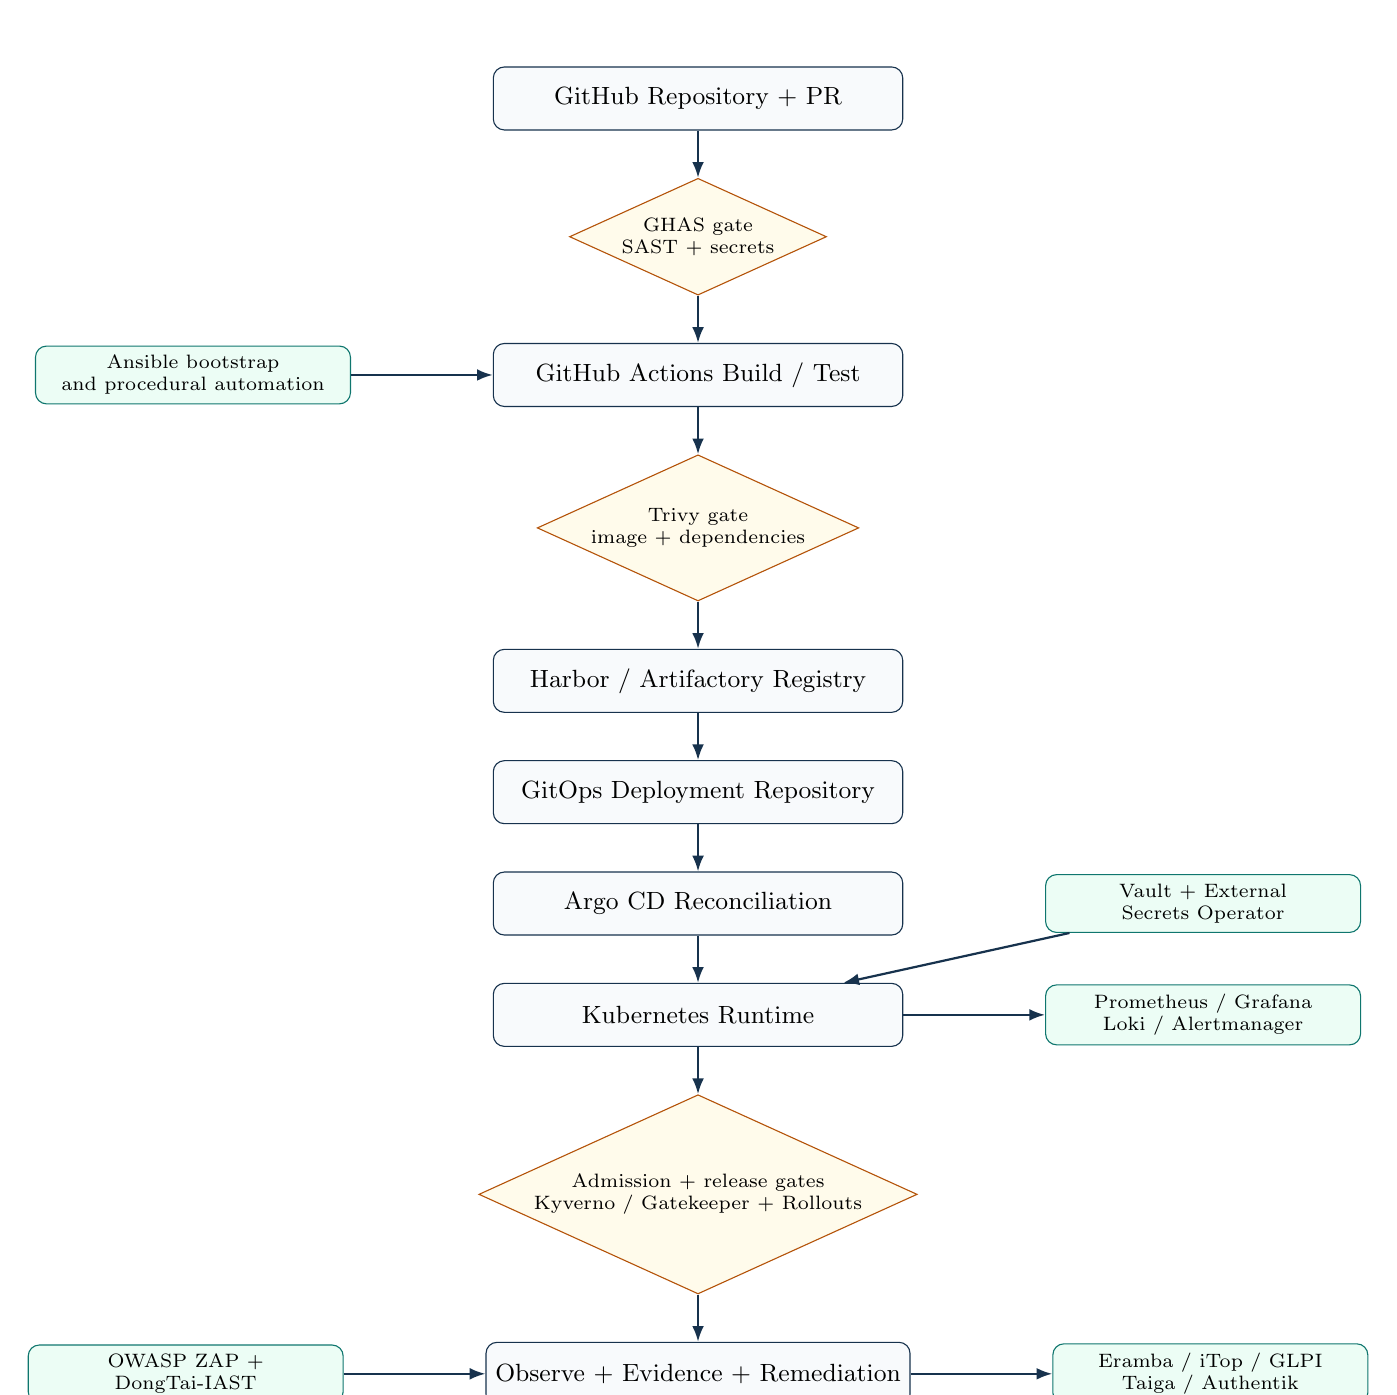
\begin{tikzpicture}[
  node distance=6mm,
  box/.style={rectangle, rounded corners, draw=Navy, fill=LightGray, align=center, minimum width=5.2cm, minimum height=8mm, font=\small},
  gate/.style={diamond, aspect=2.2, draw=Amber, fill=LightAmber, align=center, inner sep=1.2pt, font=\scriptsize},
  side/.style={rectangle, rounded corners, draw=Teal, fill=LightTeal, align=center, minimum width=4.0cm, minimum height=7mm, font=\scriptsize},
  arrow/.style={-{Latex[length=2.0mm]}, thick, draw=Navy}
]
\node[box] (repo) {GitHub Repository + PR};
\node[gate, below=of repo] (ghas) {GHAS gate\\SAST + secrets};
\node[box, below=of ghas] (ci) {GitHub Actions Build / Test};
\node[gate, below=of ci] (trivy) {Trivy gate\\image + dependencies};
\node[box, below=of trivy] (reg) {Harbor / Artifactory Registry};
\node[box, below=of reg] (gitops) {GitOps Deployment Repository};
\node[box, below=of gitops] (argocd) {Argo CD Reconciliation};
\node[box, below=of argocd] (k8s) {Kubernetes Runtime};
\node[gate, below=of k8s] (runtime) {Admission + release gates\\Kyverno / Gatekeeper + Rollouts};
\node[box, below=of runtime] (obs) {Observe + Evidence + Remediation};

\node[side, right=18mm of argocd] (secrets) {Vault + External\\Secrets Operator};
\node[side, right=18mm of k8s] (monitor) {Prometheus / Grafana\\Loki / Alertmanager};
\node[side, right=18mm of obs] (gov) {Eramba / iTop / GLPI\\Taiga / Authentik};
\node[side, left=18mm of ci] (ansible) {Ansible bootstrap\\and procedural automation};
\node[side, left=18mm of obs] (dynamic) {OWASP ZAP +\\DongTai-IAST};

\draw[arrow] (repo) -- (ghas);
\draw[arrow] (ghas) -- (ci);
\draw[arrow] (ci) -- (trivy);
\draw[arrow] (trivy) -- (reg);
\draw[arrow] (reg) -- (gitops);
\draw[arrow] (gitops) -- (argocd);
\draw[arrow] (argocd) -- (k8s);
\draw[arrow] (k8s) -- (runtime);
\draw[arrow] (runtime) -- (obs);
\draw[arrow] (secrets) -- (k8s);
\draw[arrow] (k8s) -- (monitor);
\draw[arrow] (obs) -- (gov);
\draw[arrow] (ansible) -- (ci);
\draw[arrow] (dynamic) -- (obs);
\end{tikzpicture}
\end{center}

\section{Control Loops Covered}

\begin{tabularx}{\textwidth}{L{3.1cm} Y Y}
\toprule
\textbf{Control Loop} & \textbf{Minimum Implementation} & \textbf{Evidence / Decision Output} \\
\midrule
Pull-request security gate & GHAS code scanning and secret scanning in pull-request workflow & Pass/fail status, alert context, dismissal or remediation record. \\
Build integrity gate & GitHub Actions workflow with test and security steps & Workflow run logs, build result, artifact digest. \\
Vulnerability gate & Trivy image and dependency scan before registry promotion & Vulnerability report, SBOM output, severity threshold decision. \\
Artifact promotion gate & Harbor or Artifactory repository stages & Image tag, digest, scan status, promotion record. \\
Deployment reconciliation & Argo CD syncing Kubernetes manifests from Git & Desired state, live state, drift, sync history, rollback context. \\
Runtime admission control & Kyverno or OPA Gatekeeper validating Kubernetes resources & Admission allow/deny decision and policy violation record. \\
Secret delivery control & Vault and External Secrets Operator & Secret source, sync status, access boundary, rotation support. \\
Release safety control & Argo Rollouts canary or blue-green strategy & Promotion, pause, rollback, and analysis evidence. \\
Operational health control & Prometheus, Alertmanager, Grafana, Loki & Metrics, alert history, logs, dashboards, incident context. \\
Governance and remediation control & Eramba, iTop, GLPI, Taiga & Risk/control mapping, service/CI ownership, asset context, backlog item. \\
\bottomrule
\end{tabularx}

\section{Minimum vs. Conditional vs. Deferred}

\begin{longtable}{L{3.5cm} L{2.3cm} L{8.9cm}}
\toprule
\textbf{Tool / Capability} & \textbf{Disposition} & \textbf{Rationale} \\
\midrule
\endfirsthead
\toprule
\textbf{Tool / Capability} & \textbf{Disposition} & \textbf{Rationale} \\
\midrule
\endhead
\bottomrule
\endfoot
Kubernetes & \must & Required runtime orchestrator for containerized applications. \\
Argo CD & \must & Required if Git is the deployment source of truth for Kubernetes. \\
GitHub Actions & \must & Required CI automation layer when GitHub is the source-control platform. \\
GHAS & \must & Required source security gate for CodeQL/code scanning and secret scanning. \\
Trivy & \must & Required open-source scanner for container, dependency, misconfiguration, secret, and SBOM coverage. \\
Vault + External Secrets Operator & \must & Required to avoid static secret sprawl in Kubernetes deployments. \\
Kyverno or OPA Gatekeeper & \must & Required to convert deployment policies into enforceable Kubernetes admission decisions. \\
Prometheus / Alertmanager / Grafana / Loki & \must & Required for observable, supportable release operations. \\
Ansible & \must & Required for bootstrap and procedural automation outside GitOps reconciliation. \\
Argo Rollouts & \option & Treat as minimum for production release safety; optional for early lab environments. \\
Cosign / Sigstore & \option & Add when signed image provenance, attestations, or signature verification are required.\cite{SigstoreCosignDocs} \\
OWASP ZAP + DongTai-IAST & \option & Required before production if dynamic application validation is part of the release gate. \\
Airflow / Prefect / Dagster & \defer & Data pipeline orchestration; not needed for application deployment orchestration unless scheduled data workflows are in scope.\cite{AirflowHome,PrefectQuickstart,DagsterOverview} \\
Temporal & \defer & Durable application workflow runtime; not required for ordinary deployment orchestration.\cite{TemporalWhatIs} \\
Flyte / Kubeflow / Metaflow & \defer & AI/ML workflow platforms; not part of the minimum deployment stack unless ML platform operations are in scope.\cite{FlyteOSS,KubeflowIntro,MetaflowWhatIs} \\
Docker Swarm & \defer & Redundant if Kubernetes is the selected runtime orchestrator.\cite{DockerSwarm} \\
Nomad & \defer & Useful for mixed workload estates, but redundant if the enterprise standardizes on Kubernetes.\cite{NomadWhatIs} \\
\end{longtable}

\section{Implementation Roadmap}

\subsection{Phase 1: Establish the secure delivery baseline}
\begin{enumerate}
  \item Standardize repository branch protection, required checks, and GHAS alert gates.
  \item Implement GitHub Actions workflows for build, unit tests, CodeQL/code scanning, secret scanning checks, and Trivy scans.
  \item Publish scanned images to Harbor or the existing enterprise registry using immutable tags and digests.
  \item Produce minimum release evidence: workflow run, scan summary, image digest, and target environment.
\end{enumerate}

\subsection{Phase 2: Establish GitOps deployment control}
\begin{enumerate}
  \item Create a separate GitOps repository for environment-specific deployment manifests.
  \item Use Helm charts or Kustomize overlays for environment differences.
  \item Install Argo CD and connect it to the GitOps repository.
  \item Define application sync policies, rollback approach, and drift handling rules.
\end{enumerate}

\subsection{Phase 3: Add runtime security and release safety}
\begin{enumerate}
  \item Deploy Vault and External Secrets Operator for Kubernetes secret delivery.
  \item Implement Kyverno or OPA Gatekeeper policies for allowed registries, required labels, non-root execution, resource limits, and privileged container denial.
  \item Add Argo Rollouts for canary or blue-green deployment patterns where production release safety is required.
  \item Add ZAP and DongTai-IAST validation in QA or pre-production where dynamic AppSec testing is in scope.
\end{enumerate}

\subsection{Phase 4: Close the operations and governance loop}
\begin{enumerate}
  \item Deploy Prometheus, Alertmanager, Grafana, and Loki for release health, alerts, and logs.
  \item Map services and deployment targets to iTop CIs and GLPI assets.
  \item Push risk/control evidence into Eramba where compliance or risk review is required.
  \item Create Taiga remediation items for failed gates, high-risk vulnerabilities, deployment policy violations, and post-release findings.
  \item Use Authentik for consistent SSO and group-based access across platform tools.
\end{enumerate}

\section{Selection Guardrails}

\begin{cautionbox}
\textbf{Avoid orchestration category errors.} Kubernetes is the runtime workload orchestrator. Argo CD is the GitOps reconciliation controller for Kubernetes. Ansible is procedural automation. Airflow, Prefect, and Dagster orchestrate data workflows. Temporal provides durable execution for long-running application workflows. Flyte, Kubeflow, and Metaflow belong to AI/ML workflow and platform engineering use cases. These tools are not interchangeable even when they are all described as ``orchestration'' tools.\cite{KubernetesOverview,ArgoCDHome,AnsiblePlaybooks,AirflowHome,TemporalWhatIs,KubeflowIntro}
\end{cautionbox}

\section{Operational Readiness Checklist}

\begin{multicols}{2}
\checkbox Branch protection and required checks are configured.\\
\checkbox GHAS code scanning gate is enabled.\\
\checkbox Secret scanning gate is enabled.\\
\checkbox Trivy scan threshold is documented.\\
\checkbox Registry promotion rules are documented.\\
\checkbox Kubernetes namespaces and RBAC are defined.\\
\checkbox Argo CD app ownership is defined.\\
\checkbox Helm or Kustomize standards are documented.\\
\checkbox Vault secret paths and access policies are defined.\\
\checkbox External Secrets Operator sync model is tested.\\
\checkbox Kyverno or Gatekeeper policies are versioned.\\
\checkbox Production rollout strategy is defined.\\
\checkbox Prometheus alerts are mapped to support queues.\\
\checkbox Grafana dashboards cover deployment health.\\
\checkbox Loki log retention is documented.\\
\checkbox Eramba evidence mapping is defined.\\
\checkbox iTop / GLPI ownership mapping is defined.\\
\checkbox Taiga remediation workflow is defined.\\
\checkbox Authentik groups map to platform roles.\\
\checkbox Rollback and break-glass procedures are tested.\\
\end{multicols}

\section{Recommended Minimum Decision}

\begin{riskbox}
\textbf{Final decision.} Adopt \tool{Kubernetes + Argo CD + GitHub Actions + GHAS + Trivy + Harbor/Artifactory + Vault + External Secrets Operator + Kyverno or OPA Gatekeeper + Prometheus/Grafana/Loki/Alertmanager + Ansible}. Integrate release evidence and findings into \tool{Eramba}, \tool{iTop}, \tool{GLPI}, and \tool{Taiga}, with \tool{Authentik} as the access-control front door. Add \tool{Argo Rollouts} for production release safety. Add \tool{Cosign/Sigstore} when image signing, provenance, or attestation verification is required.
\end{riskbox}

\begin{thebibliography}{99}
\bibitem{GitHubActions} GitHub Docs. \emph{GitHub Actions documentation}. Available: \url{https://docs.github.com/actions}
\bibitem{GHASCodeScanning} GitHub Docs. \emph{About code scanning}. Available: \url{https://docs.github.com/en/code-security/code-scanning/introduction-to-code-scanning/about-code-scanning}
\bibitem{GHASSecretScanning} GitHub Docs. \emph{About secret scanning}. Available: \url{https://docs.github.com/en/code-security/secret-scanning/introduction/about-secret-scanning}
\bibitem{TrivyDocs} Aqua Security. \emph{Trivy Documentation}. Available: \url{https://trivy.dev/latest/}
\bibitem{HarborDocs} Harbor Documentation. \emph{Harbor Introduction}. Available: \url{https://goharbor.io/docs/}
\bibitem{KubernetesOverview} Kubernetes Documentation. \emph{Overview}. Available: \url{https://kubernetes.io/docs/concepts/overview/}
\bibitem{ArgoCDHome} Argo CD Documentation. \emph{Argo CD - Declarative GitOps CD for Kubernetes}. Available: \url{https://argo-cd.readthedocs.io/en/stable/}
\bibitem{ArgoCDDeclarative} Argo CD Documentation. \emph{Declarative Setup}. Available: \url{https://argo-cd.readthedocs.io/en/stable/operator-manual/declarative-setup/}
\bibitem{HelmDocs} Helm Documentation. \emph{Helm}. Available: \url{https://helm.sh/docs/}
\bibitem{KustomizeDocs} Kubernetes Documentation. \emph{Kustomize}. Available: \url{https://kubernetes.io/docs/tasks/manage-kubernetes-objects/kustomization/}
\bibitem{AnsiblePlaybooks} Ansible Community Documentation. \emph{Working with playbooks}. Available: \url{https://docs.ansible.com/projects/ansible/latest/playbook_guide/playbooks.html}
\bibitem{AnsibleRolling} Ansible Community Documentation. \emph{Playbook Example: Continuous Delivery and Rolling Upgrades}. Available: \url{https://docs.ansible.com/projects/ansible/latest/playbook_guide/guide_rolling_upgrade.html}
\bibitem{VaultDocs} HashiCorp Developer. \emph{What is Vault?}. Available: \url{https://developer.hashicorp.com/vault/docs/what-is-vault}
\bibitem{ExternalSecretsDocs} External Secrets Operator Documentation. \emph{Introduction}. Available: \url{https://external-secrets.io/latest/}
\bibitem{KyvernoDocs} Kyverno Documentation. \emph{Introduction}. Available: \url{https://kyverno.io/docs/introduction/}
\bibitem{GatekeeperDocs} Open Policy Agent Gatekeeper Documentation. \emph{Gatekeeper}. Available: \url{https://open-policy-agent.github.io/gatekeeper/website/}
\bibitem{ArgoRolloutsDocs} Argo Rollouts Documentation. \emph{Argo Rollouts}. Available: \url{https://argo-rollouts.readthedocs.io/en/stable/}
\bibitem{PrometheusDocs} Prometheus Documentation. \emph{Overview}. Available: \url{https://prometheus.io/docs/introduction/overview/}
\bibitem{AlertmanagerDocs} Prometheus Documentation. \emph{Alertmanager}. Available: \url{https://prometheus.io/docs/alerting/latest/alertmanager/}
\bibitem{GrafanaDocs} Grafana Documentation. \emph{Grafana documentation}. Available: \url{https://grafana.com/docs/grafana/latest/}
\bibitem{LokiDocs} Grafana Loki Documentation. \emph{Grafana Loki}. Available: \url{https://grafana.com/docs/loki/latest/}
\bibitem{ZAPDocs} OWASP ZAP Documentation. \emph{ZAP Documentation}. Available: \url{https://www.zaproxy.org/docs/}
\bibitem{DongTaiDocs} DongTai Documentation. \emph{DongTai}. Available: \url{https://doc.dongtai.io/}
\bibitem{ErambaDocs} Eramba Documentation. \emph{Documentation}. Available: \url{https://www.eramba.org/documentation/}
\bibitem{iTopDocs} iTop Documentation. \emph{iTop Documentation}. Available: \url{https://www.itophub.io/wiki/page?id=latest:start}
\bibitem{GLPIDocs} GLPI Documentation. \emph{GLPI Documentation}. Available: \url{https://glpi-install.readthedocs.io/en/latest/}
\bibitem{TaigaDocs} Taiga Documentation. \emph{Taiga Docs}. Available: \url{https://docs.taiga.io/}
\bibitem{AuthentikDocs} Authentik Documentation. \emph{Authentik Documentation}. Available: \url{https://docs.goauthentik.io/}
\bibitem{SigstoreCosignDocs} Sigstore Cosign Documentation. \emph{Cosign}. Available: \url{https://docs.sigstore.dev/cosign/}
\bibitem{AirflowHome} Apache Airflow Documentation. \emph{What is Airflow?}. Available: \url{https://airflow.apache.org/docs/apache-airflow/stable/index.html}
\bibitem{PrefectQuickstart} Prefect Documentation. \emph{Quickstart}. Available: \url{https://docs.prefect.io/v3/get-started/quickstart}
\bibitem{DagsterOverview} Dagster Documentation. \emph{Overview}. Available: \url{https://docs.dagster.io/}
\bibitem{TemporalWhatIs} Temporal Documentation. \emph{What is Temporal?}. Available: \url{https://docs.temporal.io/temporal}
\bibitem{FlyteOSS} Flyte OSS Documentation. \emph{User Guide / Flyte OSS}. Available: \url{https://docs.flyte.org/}
\bibitem{KubeflowIntro} Kubeflow Documentation. \emph{Introduction}. Available: \url{https://www.kubeflow.org/docs/started/introduction/}
\bibitem{MetaflowWhatIs} Metaflow Documentation. \emph{What is Metaflow}. Available: \url{https://docs.metaflow.org/introduction/what-is-metaflow}
\bibitem{DockerSwarm} Docker Docs. \emph{Swarm mode}. Available: \url{https://docs.docker.com/engine/swarm/}
\bibitem{NomadWhatIs} HashiCorp Nomad Documentation. \emph{What is Nomad?}. Available: \url{https://developer.hashicorp.com/nomad/docs/what-is-nomad}
\end{thebibliography}

\end{document}
